\section{Optimisations}\label{sec:rw:sgfd:optim}
L'héritage des connaissances du domaine des systèmes relationnels a été central sur la conception des systèmes de gestion de flux de données. Concernant l'optimisation du traitement des requêtes, il existe plusieurs techniques concernant les SGBD. Dans cette section, nous présenterons les stratégies d'optimisations appliqués aux SGFD. Tout d'abord, nous rappellerons les grands principes du traitement des requêtes des bases de données. Par la suite, nous nous concentrerons sur les points spécifiques à la nature des requêtes continues. Enfin, nous présenterons des principes d'implémentation des algorithmes spécifiques aux opérateurs.

\subsection{Optimisation dans les SGFD-R}
Ainsi, afin de mieux analyser les optimisations de la gestion de flux, il devient important d'investiguer plus en détail le fonctionnement de la gestion de base de données.

\subsubsection{Le problème dans sa globalité}
Le processus d'optimisation usuel en gestion de base de données est maintenant établie et répendue~\cite{Ioannidis:optimization}. Une requête en gestion de base de donnée est soumise par un langage déclaratif tel que \textit{SQL}. A partir de cette expression, s'enchaine une série d'opération qui permettra l'exécution de celle-ci. La figure \ref{fig:rw:sgfd:optim:processus} décrit le processus complet nécessaire à l'aboutissement de ce traîtement. 
\begin{figure}[h]
\centering
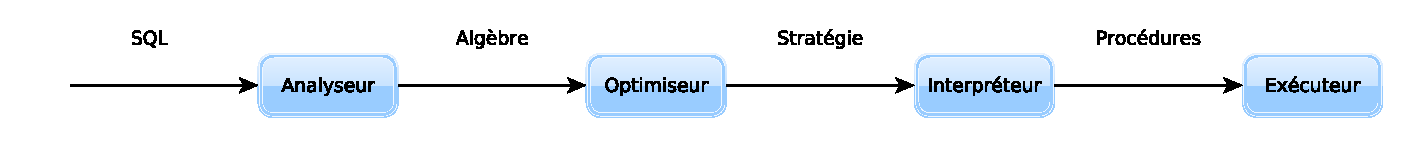
\includegraphics[width=0.9\textwidth]{rw-sgfd-optimsgbd}
\caption{Processus de traitement de requête dans un SGBD-R}\label{fig:rw:sgfd:optim:processus}
\end{figure}

Plusieurs modules permettent d'exécuter cette série d'opérations :
\begin{itemize}
    \item \textbf{Analyseur} : Prend en entrée une requête textuelle et fournit en sortie un arbre de requête écrit dans un format interne équivalent à de l'algèbre relationnelle. Ce module ne fait que traduire la grammaire du SQL par des règles prédéfinies.
    \item \textbf{Optimiseur} : Prend cet arbre de requête et fournit un autre arbre de requête, agrémenté d'indication de méthodes physique à utiliser. Le tout forme une stratégie d'exécution qui ne sera pas modifiée par la suite. Le but de cette étape est de fournir la stratégie qui fournit un résultat identique à ce que l'arbre initial était avec un coût moindre.
    \item \textbf{Interpréteur} : Récupère la stratégie d'exécution et instancie les procédures d'exécution. Le tout sera envoyé à l'\textbf{exécuteur} qui manipulera ces procédures afin de produire le résultat final.
\end{itemize}
L'optimiseur étant bien entendu le module le plus complexe car il possède et utilise beaucoup de connaissance et de résultats sur la gestion de données. Ce composant s'est prouvé indispensable dans la pratique car une bonne stratégie de traitement changera la plupart du temps de complexité ce qui transformera une requête pouvant être exécutée en plusieurs heures en moins d'une seconde.

Le problème est que l'espace des stratégies possibles pour exécuter une requête classique est potentiellement de cardinalité factorielle en fonction du nombre d'opérateurs et de méthodes d'exécutions disponibles (surtout s'il y a des jointures). Ainsi, il faut guider l'exploration et utiliser des techniques de programmation dynamique pour éliminer rapidement les branches trop coûteuses.

L'optimisation de requête se découpe en deux sections : l'optimisation logique (i.e. sélection du meilleur arbre d'opérateur théorique) et l'optimisation physique (choix des meilleurs algorithmes).

\subsubsection{Optimisation Logique}
L'espace algébrique est très large car les équivalences sur l'algèbre relationnelle sont très larges et permissives. Par exemple, une sélection sur une jointure $\sigma (R_1 \Join R_2)$ peut traverser l'opérateur binaire si sa condition ne concerne qu'une branche : $R_1 \Join \sigma R_2$. Ainsi, pour un arbre de requête, il peut y avoir des millions de requêtes équivalentes avec des permutations ou des ajouts d'opérateurs. Des heuristiques sont ainsi sélectionnées pour réduire cet espace tout en restant efficace~\cite{Ioannidis:optimization}. Le critère principal d'optimisation étant minimiser la taille des résultats intermédiaires. Voici les règles classiques :
\begin{itemize}
    \item[\textbf{R1}~:] \textit{La sélection et la projection n'introduisent pas de coût supplémentaires et sont traités à la volée}. Les sélections doivent être exécutés au moment de la première lecture sur la relation. Les projections doivent se faire en même temps que le résultat d'un autre opérateur.
    \item[\textbf{R2}~:] \textit{Les produits cartésiens ne doivent jamais être formés sauf si la requête elle-même en demande}. Seules les jointures peuvent combiner des relations.
    \item[\textbf{R3}~:] \textit{L'opérande interne (partie droite) de chaque jointure est une relation originelle, et non un résultat intermédiaire}.
\end{itemize}

La règle R1 est utilisée pour minimiser la taille des résultats intermédiaires. La règle R2 supprime toute possibilité de recours fatal aux algorithmes de boucles imbriquées sachant qu'un autre plan pouvait utiliser à chaque fois des jointures plus efficaces.

La règle R3 n'est pas toujours choisie car même si elle réduit beaucoup les possibilités car elle restreint les ordres de jointures, elle risque de supprimer l'arbre optimal dans plusieurs cas. En effet, les arbres de requêtes ne pourront pas être des arbres équilibrés car l'opérande droite doit être une relation native, or un arbre déséquilibré peut introduire des surcoûts du fait que les jointures supérieur doivent joindre une grande relation avec un résultat intermédiaire. Toutefois, il existe des raisons à cette règle. Tout d'abord, le fait d'avoir des relations natives permet l'utilisation d'index. De plus elle permet de faire un traitement total des requêtes en mode \textit{pipeline}\footnote{L'exécution en \textit{pipeline} permet de traiter un n-uplet dès sa lecture, notons que cela s'apparente à du traitement de flux. L'avantage étant que le processeur étant moins coûteux que les entrées-sorties, on peut rentabiliser l'attente de lecture en traitement de requête.}.

En parcourant l'espace algébrique des requêtes équivalentes vérifiant R1-3, le nombre de plans devient raisonnablement faible. Pour le reste des recherches, il sagit principalement de choisir l'ordre des jointures. Comme la jointure est symétrique $R_1 \Join R_2 = R_2 \Join R_1$ alors dans le cas de multiples jointures (courant en gestion de base de données), il faut choisir l'ordre le plus pertinent qui minimisera la taille des résultats intermédiaires. Cette recherche se fera conjointement avec l'optimisation physique du fait de son impact sur les algorithmes.

\subsubsection{Optimisation Physique}
L'optimisation physique correspond au parcours de l'espace des méthodes disponibles pour chaque plan de requête et à l'évaluation quantitative de chacune de celles-ci. L'espace des méthodes fournit plusieurs implémentation pour un opérateur. Par exemple pour la jointure :
\begin{itemize}
    \item \textbf{Boucles imbriqués} : Implémentation la plus directe de la jointure. Cet algorithme ne requiert aucune condition sur les relations d'entrées.
    \item \textbf{Jointure fusion} : Se base sur le fait que les deux relations sont triés sur l'attribut de jointure à l'avance. Ainsi la jointure est plus facile à effectuer. Elle est régulièrement utilisée avec des index triés comme les arbres B+~\cite{Comer:btree}. Des opérateurs de tri pourront être déployés si ces index sont absent.
    \item \textbf{Jointure hachée} : Se base sur le fait que les deux relations sont hachées sur l'attribut de jointure. Ainsi la jointure se fait sur les index de hachages de cardinalité réduite et d'accès rapide.
\end{itemize}

Pour chaque relation, il existe deux moyens principaux d'accéder à un n-uplet :
\begin{itemize}
 \item \textbf{Scan} : Parcours strict de la relation ou d'un l'index pour trouver les n-uplets vérifiant une condition de sélection.
 \item \textbf{Probe} : Demande directement aux procédures d'index de renvoyer les tuples vérifiant une condition de sélection.
\end{itemize}

Ainsi, il est possible de faire des boucles imbriqués suffisamment performantes en utilisant des accès optimisés aux relations. Bien évidemment certaines sélections sont impossibles via les procédures d'index. Par exemple, il est impossible de demander à un index haché de faire une sélection avec un opérateur de comparaison tel que \enquote{$\leq$}.

L'évaluation de chacune de ces méthodes passe par un coût global de l'exécution basé sur des statistiques. Ces statistiques aideront à quantifier la taille des résultats intermédiaires. Pour cela, il est nécessaire de faire des calculs de sélectivité~\cite{Selinger:selectivity}. Ces calculs permettent d'évaluer le ratio d'n-uplet qui valident une sélection. Par exemple, en l'absence d'information complémentaire, une sélectivité de 10\% est appliquée par défaut. Par la suite chaque algorithme est capable de quantifier son coût en fonction de ces sélectivités et des cardinalités des entités manipulées.

Suivant les capacités du système et la taille de la requête, le système pourra réordonner les jointures pour optimiser les algorithmes. La recherche dans cet espace de méthode se base sur la programmation dynamique. Elle permet de faire une recherche exhaustive sans être extrêmement coûteuse (par des procédures de \textit{branch \& bound} usuelles).

\paragraph*{Optimisation de la recherche}
La recherche exhaustive peut être très coûteuse si les jointures sont nombreuses car l'espace des stratégies devient large, ce qui peut être long à calculer. Une approche heuristique est nécessaire pour avoir un temps de calcul qui permette un lancement rapide de la requête. 

Plusieurs approches existent, la plus connue reste basée sur la marche aléatoire sur le graphe des stratégies possibles. Celle-ci parcourt le graphe aléatoirement en reculant si le coût est devenu trop important. Une autre approche intéressante étant l'utilisation d'algorithmes génétiques pour résoudre ce problème. \textit{Postgres} utilise l'optimiseur \textit{Genetic Query Optimizer (GEQO)}~\cite{Postgres:geqo} si le nombre de jointure dépasse une certaine limite.

L'optimisation a été prouvée comme un problème NP-complet~\cite{Ibaraki:join} (même avec seulement les boucles imbriqués) ainsi certains efforts se sont concentré sur la résolution de sous cas importants, notamment boucles imbriqués et jointure hachée seulement.

\paragraph*{Base de données parallèles}
L'optimisation en prenant en compte des modèles de calculs parallèles est un problème encore ouvert. Toutefois, des approximations efficaces se basent sur les optimisations à deux phases. Tout d'abord, le système recherche la solution optimale comme vu précédemment. Par la suite, il cherche le meilleur ordonnancement. Les deux domaines ont été suffisamment couverts pour obtenir des résultats satisfaisants.

\paragraph*{Distribution du calcul}
La distribution du calcul est un problème différent des bases parallèles dans le sens où il existe plusieurs unités d'évaluation complètement indépendantes. Le problème toutefois se résout principalement en quantifiant la distribution du calcul à l'intérieur de l'espace des méthodes. L'espace de recherche sera toutefois plus grand et il faudra faire attention à avoir un optimiseur performant pour ne pas avoir de surcoût avant l'exécution.

\paragraph*{L'optimisation sémantique}
Supposons la présence d'une base de connaissance en parallèle de la base de donnée. Il est alors possible de raisonner sur les conditions de sélections notamment, afin d'amener plus ou moins de restriction à la requête. Les calculs d'inférence de concepts, comme vus en section~\ref{sec:rw:supervision:contexte}, permettent d'extraire des conditions plus restrictives mais équivalentes. Le problème étant d'avoir une base de connaissance suffisamment exploitable car une erreur de raisonnement pourrait supprimer potentiellement des résultats. De plus, les calculs d'inférences peuvent être lourds et ne doivent pas rendre le traitement de requête trop lourd. Cette approche commence a être exploitée en gestion de flux de données aussi grâce à des méta-données~\cite{Ding:semantic}.

\subsection{Optimisation spécifique de la gestion de flux}
L'infrastructure de traitement des flux est sensiblement différente à la gestion des bases de données. Ainsi, des optimisations plus spécifiques sont applicables dans ce contexte concernant : le mode de traitement des requêtes, la gestion de la charge sur le long terme, le partage des requêtes, l'ordonnancement et enfin le routage pour les infrastructures distribués. Nous pouvons remarquer que toutes ces optimisations ont été explorées premièrement dans le domaine des systèmes de base de données. Toutefois, ils prennent plus d'ampleur dans ce contexte.

\subsubsection{Calcul incrémental}
Le principe fondateur de la gestion de flux étant que les données arrivent de manière continue. Comme présenté dans la section~\ref{sec:rw:sgfd:modeles}, les premiers traitement de flux~\cite{Terry:tapestry} étaient considérés comme des traitements particuliers sur des relations sans suppression ou mise à jour.

De façon plus générale, en se plaçant dans l'algèbre \textit{ACO} : Soit $R$ une relation, au lieu de calculer une requête sur $R(\tau)$, il est possible de considérer les \textit{delta} de cette relation : $\Delta_R^+(\tau) = R(\tau)-R(\tau-1)$ et $\Delta_R^-(\tau) = R(\tau-1)-R(\tau)$. Comme le traitement des fenêtres, par exemple, peut fournir directement ces différences : il n'y a donc pas de surcoût à l'utilisation d'un tel procédé. Comme la cardinalité des $\Delta$ est souvent minime face à celle de la relation totale. Il devient intéressant de travailler avec ces données.
\subsubsection{Load-shedding}
Contrairement aux approches classiques de gestion de base de données, il est important de voir que l'optimisation n'est pas toujours de pouvoir fournir les résultats exacts aux requêtes. L'objectif étant de fournir les résultats les plus pertinents possibles avec des contraintes d'espace mémoire, de temps de réponse ainsi que de charge réseau. En effet, comme la gestion de flux fonctionne de manière continue, une congestion dans le processus de traitement impliquera des retards et des complications pouvant aller jusqu'à une saturation du moteur.

L'idée du \textit{load-shedding} est de pouvoir abaisser ou limiter le taux de n-uplet au nombre suffisant pour pouvoir traiter sans introduire de retard. Dans les travaux fondateurs~\cite{Tatbul:window,Tatbul:load-shedding}, l'idée est de pouvoir surveiller le traitement des requêtes afin de reconnaitre les points d'engorgements et d'y implanter des opérateurs de shedding. Afin de garantir un certain taux de réussite, la politique qui sera utilisée pour le \textit{load-shedding} sera dirigée par une \textit{QoS}\footnote{QoS : Quality of Service} déterminant quelles données sont utiles. En effet, en prenant en entrée un graphe représentant \textit{valeur} $\mapsto$  \textit{taux de suppression acceptable}. Par exemple, dans le cadre d'une surveillance d'incendie, le taux de \textit{shedding} pour les températures inférieure à 20ºC pourra être très fort de part et d'autre du systèmes pour ce genre de données. Le critère de sélection afin d'autoriser la suppression d'une données peut se faire de façon différentes :
\begin{itemize}
 \item Par un histogramme et un choix sur le nombre de tuple résultant~\cite{Han:join}
 \item Par un calcul probabiliste pour privilégier un flux plutôt qu'un autre pour sa productivité~\cite{Han:join}
 \item Par des raisonnements sur l'age du n-uplet~\cite{Srivastava:join}
\end{itemize}


\subsubsection{Multi-Query Optimization (MQO)}
Aussi connu sous le nom de \textit{Global Query Optimization}. Cette optimisation profite des exécutions parrallèles pour éviter la redondances de traitement et une économie de ressources. Elle est issue du monde des SGBD~\cite{Sellis:mqo} et permet de répondre à plusieurs requêtes en même temps en utilisant des parties communes (classiquement, lorsque seules les clauses de sélection sont différentes). L'idée est toutefois peu exploitée car il faut pouvoir soumettre plusieurs requêtes en même temps et les gestions de caches ont permis de faire de bon résultat pour ce genre de requêtes. 

Dans le monde des flux de données, cette optimisation est largement reconnue comme importante. Les requêtes durant dans le temps, de façon potentiellement infinie, le nombre d'exécution concurrente sera donc très grand. Ainsi, partager les ressources des requêtes devient une façon d'optimiser grandement les requêtes. Plusieurs points interviennent ici.
\begin{itemize}
 \item Tout d'abord l'existence des \textit{m-op} (multi-operators)~\cite{Hong:mqo}. Ces opérateurs permettent de regrouper plusieurs opérateurs en un seul permettant d'éviter des duplicatas de n-uplets. Un exemple classique étant de grouper deux sélections sur un flux commun en une seule. Ainsi, si un n-uplet vérifie les deux sélections, un seul n-uplet sera fournit avec l'indication qu'il appartient aux requêtes 1 et 2. Cette optimisation permet de faire des requêtes en utilisant les définitions de flux fragmentés.
 \item Grande disponibilité des ressources. Chaque opérateur utilise des ressources et peut potentiellement les partager avec d'autres. Cependant, ces ressources ne sont peut-être pas utiles à partager car elles sont trop précises. Dans plusieurs travaux~\cite{Arasu:resource}, le calcul des agrégations sur fenêtres peut être partagé. En découpant la mémoire par bloc de façon intelligente, on peut partager les ressources afin d'économiser de la place mémoire.
\end{itemize}

Un problème ouvert reste de savoir si les optimisations locales (optimisation algébrique) gêneront les optimisations globales. Une requête ne possède pas qu'une seule optimisation au début de son traitement. En effet, si une nouvelle requête arrive et qu'en changeant légèrement la structure de la première, il est possible d'obtenir un partage, alors il est probable que ce nouveau plan soit le bon. L'adaptabilité d'une requête est donc importante.

\subsubsection{Ordonnancement}
Comme les requêtes s'exécutent en parallèle, la notion d'ordonnancement entre en compte. Afin d'éviter les engorgements, ou pour donner plus de priorité à une partie de la requête, l'ordonnanceur doit cadancer les unités de traitement pour fournir des résultats conformes à la qualité attendue. Par exemple, une requête importante (type alerte) peut exprimer des contraintes forte de \textit{latence}. A l'inverse, une requête d'observation passive aura des contraintes plus faible. Plusieurs stratégies ont été proposés~\cite{Babcock:chain, Jiang:scheduling} afin de garantir le meilleur temps de réponse en utilisant le moins de resources possibles.

\subsubsection{Routage}
Le problème du routage est un problème très connu du domaine des réseaux de capteurs où les contraintes de traitement sont si fortes au niveau de la transmission de données que les routages sont importants. Pour le traitement en flux de grandes quantités de données, des optimisations de routages rentrent en compte sur le calcul de jointure par exemple~\cite{Zhou:pmjoin}. En effet, il nous faut savoir s'il vaut mieux effectuer une opération lourde et ayant une sélectivité peut-être grande (>1) de façon distribuée avec transfert réseaux ou groupés mais plus chargés en traitement. 

De façon similaire, le coût (notamment énergétique) est analysé afin de fournir un routage au moment du placement de la requête~\cite{Galpin:snee} ou à l'exécution~\cite{Madden:tinydb}.

\subsection{Optimisation d'algorithmes}

\subsubsection{Jointures}
Comme présenté précédemment, la jointure en flux n'est pas aussi simple qu'une jointure au sens base de données car elle introduit la notion de fenêtre. Beaucoup de travaux~\cite{Han:join, Srivastava:join, Law:join} se sont portés sur les jointures similaires à $I_S (S_1[W_1] \Join ... \Join S_n[W_n])$ et bien souvent avec des fenêtres identiques. Car l'implémentation de ceci requiert a priori une quantité non bornée de mémoire. De plus le traitement d'un n-uplet prendra du temps et il faudra pouvoir fournir le résultat sans retard par rapport aux flux d'entrées. L'utilisation des procédures de \textit{load-shedding} est aussi utile dans ce cas.

L'utilisation d'index, comme couramment appliqué en SGBD, est désormais plus délicat car les données sont constamment actualisées. Le point crucial de l'index étant que le surcoût introduit au moment de l'insertion d'une donnée est amorti par le nombre de fois où la donnée sera interrogée. Il est toutefois important de noter que les optimisations présentes dans le calcul de jointures relationnelles en mode \textit{pipeline}~\cite{Gajski:pipeline} sont ici applicables telles que le \textit{symetric hash join}~\cite{Wilschut:symetricjoin} souvent appliqué.

D'autres optimisations ont été abordés sur la distribution du calcul~\cite{Zhou:pmjoin}. En effet, le coût engendré par les échanges fait que le calcul de la distribution des opérateurs devient importante. Dans cette optimisation, il est important de prendre en compte le partitionnement de la charge du flux par rapport au domaine des attributs de jointures. En effet, un attribut pourra avoir un débit très faible sur une valeur comparé à un autre qui sera bien plus présent.

Enfin, de façon un peu plus particulière, il est intéressant de noter les optimisations dans des contextes particuliers tels que le P2P (avec une DHT)~\cite{Palma:p2p}. Le calcul de la jointure peut se faire sur plusieurs noeuds afin de mieux distribuer le traitement.

\subsubsection{Fenêtrage et agrégations}
Nous nous intéressons maintenant particulièrement aux traitements de requêtes d'agrégations de classe $I_S(G(S[W]))$. Les travaux les plus conséquents se focalisent sur le fait de calculer de façon approximative des opérations de comptage et de quantile en mémoire limité~\cite{Arasu:window}. Ce comptage permet d'effectuer les autres statistiques en quantité restreinte~\cite{Datar:stats}, comme par exemple : 
\begin{itemize}
 \item Min/Max/Sum/Avg 
 \item Moyennes
 \item Tables de hachages
 \item Histogrammes
 \item Nombre de valeurs distinctes
\end{itemize}

L'approche est principalement mathématique et probabiliste. Par exemple, en se fixant une tolérance $\eps$, il est possible d'obtenir un résultat dans une quantité de mémoire prévisible.

\subsection{Synthèse}
Profitant des caractéristiques particulières en terme de contraintes de rapidité d'exécution, il y a eu de nombreux développement concernant l'optimisation dans les SGFD. Les plus gros efforts se sont concentrés sur le calcul d'algorithmes incrémentaux, ainsi que sur l'utilisation de réponses approximatives. Seulement quelques approches comme~\cite{Galpin:snee,Kramer:semantics} s'intéressent au fait de faire une optimisation de plan de requête (logique puis physique). Toutefois, le manque de connaissance dans le domaine théorique de la gestion de flux de données fait que les équivalences de requêtes sont peu nombreuses en dehors des usuelles~\cite{Slivinskas:temporal,Arasu:stream}.

Ainsi, comparé à l'optimisation des SGBD, seules les règles évidentes telles que l'application de projections au plus près des sources sont faites dans l'optimisation logique. Peu de parcours de plans de requêtes et de stratégies d'exécutions équivalentes n'est appliqué. De même, la prise en considération des autres requêtes pour le partage de résultat intermédiaire est une stratégie efficace. Toutefois, cette opération est principalement faite de façon manuelle à l'installation d'une nouvelle requête. Seuls des travaux comme RUMOR~\cite{Hong:mqo} recherchent à fusionner le nouveau plan de requête avec un autre (sous condition strictes).

Nous pouvons donc conclure que l'optimisation en gestion de flux de données a été grandement travaillée et a produit de multiples techniques. Toutefois, une utilisation de ces techniques pour faire une \textbf{recherche d'optimisation globale} sans intervention de l'utilisateur est encore limitée notamment du au manque de connaissance théorique.
